\section{Durchführung}

\begin{figure}
    \centering
    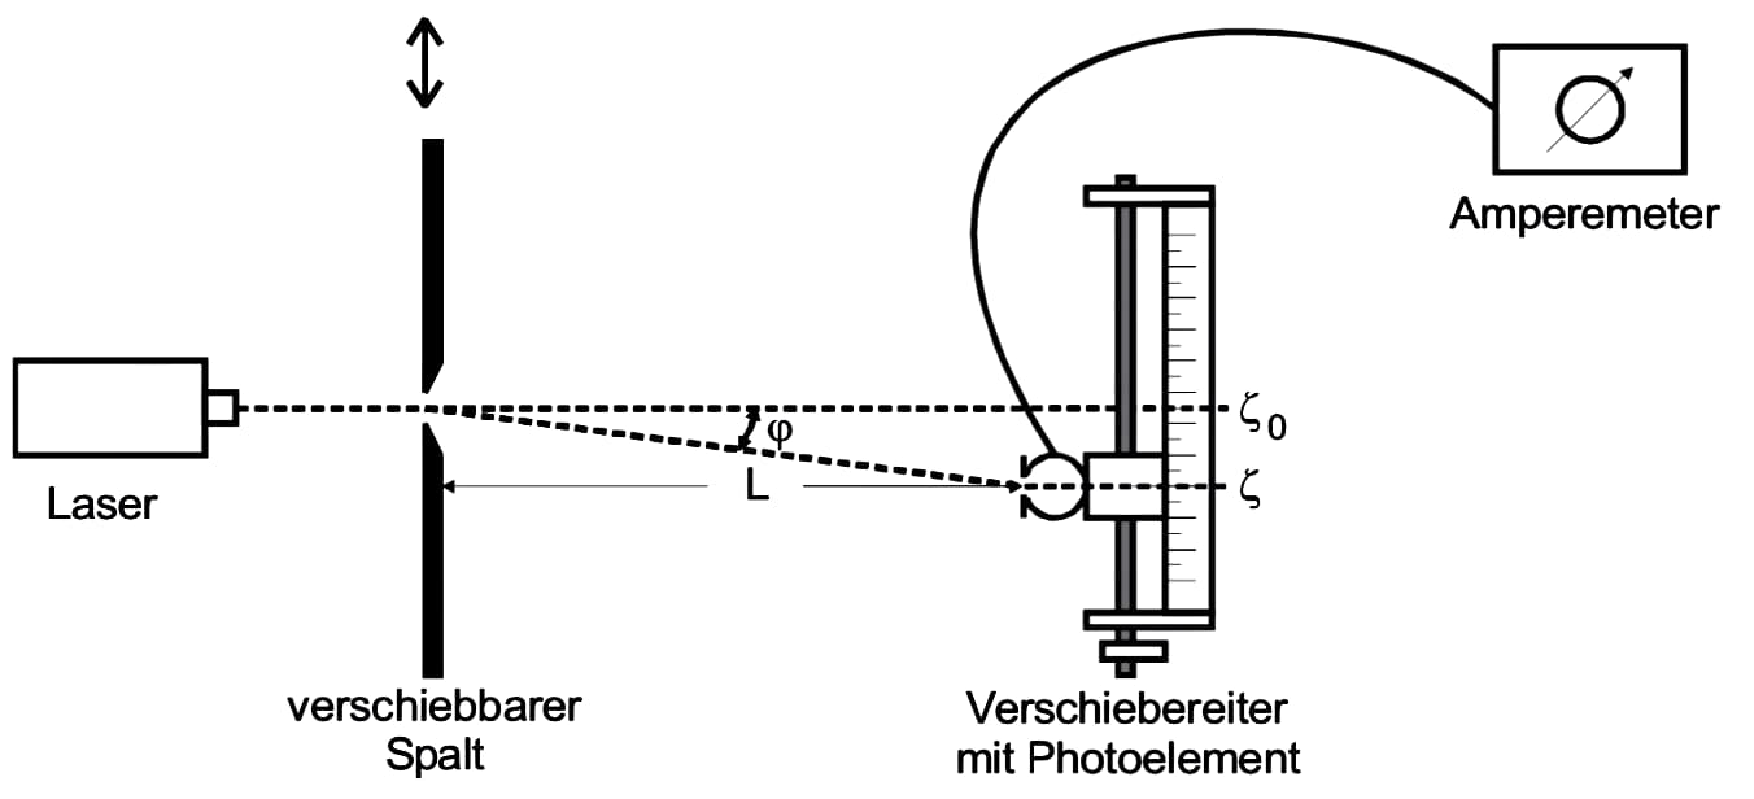
\includegraphics[scale=0.5]{content/Beugung Aufbau.pdf}
    \caption{Hier zu sehen ist die Skizzierung von dem Aufbau, welches im Experiment verwendet wurde.}
    \label{fig:skaufbau}
\end{figure}

\begin{figure}
    \centering
    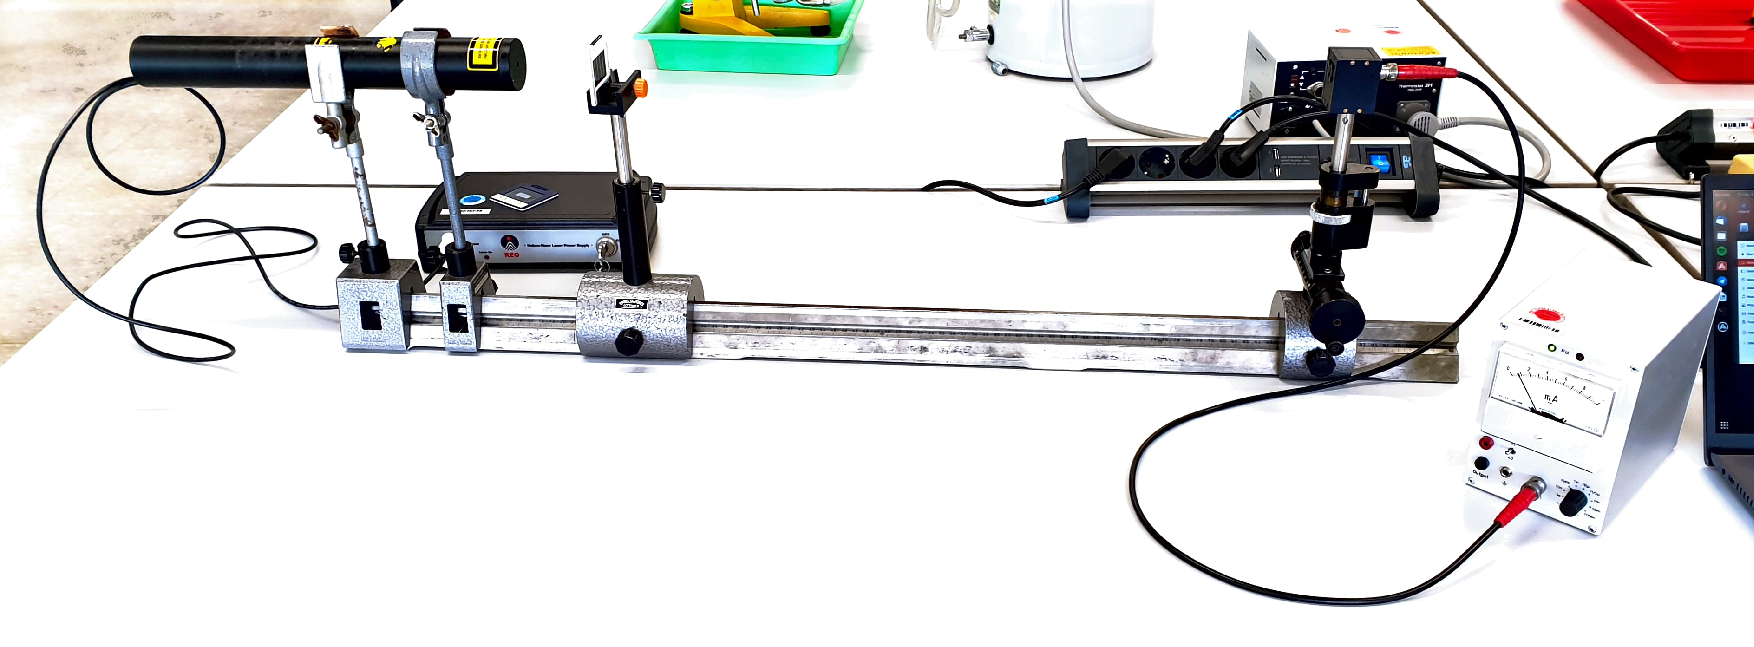
\includegraphics[scale=0.5]{content/Beugung Aufbau Real.pdf}
    \caption{Dies ist ein Foto von dem Aufbau, welcher für diesen Versuch verwendet wurde.}
    \label{fig:reaufbau}
\end{figure}

Zunächst wird mit dem Einfach-Spalt eine Beugungsfigur punktweise ausgemessen. Hierzu wird ein Einfach-Spalt mit 75 Mikrometer Spaltbreite in 62,5 Zentimeter Abstand zum Detektor gestellt und so positioniert, dass dieser sich im Maximum  der Intensität befindet. Nun wird der Detektor von einem Laser mit einer Wellenlänge von 633 Nanometern beschienen. Der Detektor wird daraufhin nach jeder Messung um 300 Mikrometer senkrecht zur Abstandslinie zwischen Spalt und Detektor für \(\phi\) = 0 verschoben, bis 50 Messungen erhalten sind. Der Detektor wurde mit einer Noise von acht Nanoamperen eingestellt.\\
Im Nachhinein wird der Einzelspalt durch den Doppelspalt ausgetauscht und das Prozedere wiederholt. Die Spaltenbreite beträgt nun 150 Mikrometer und der Abstand beider Spalten beträgt 250 Mikrometer. Die Schrittweite ist nun 100 Mikrometer. Die restlichen Einstellungen bleiben gleich.

\label{sec:Durchfuehrung}
